\documentclass[9pt]{beamer}
\usetheme{Antibes}
\useinnertheme{rectangles}
\useoutertheme{infolines}
\usepackage[utf8]{inputenc}
\usepackage[T1]{fontenc}
\usepackage[ngerman]{babel}

% patch the look of +, = in arev
\usefonttheme{serif} 

\usepackage{arev}
\usepackage{amsmath}
\usepackage{amssymb}

\setbeamertemplate{footline}{%
\begin{beamercolorbox}[ht=3.0ex,dp=1ex]{title in head/foot}
\hfill\footnotesize\insertpagenumber\enspace\enspace\end{beamercolorbox}}

\definecolor{bluegreen1}{rgb}{0.0,0.20,0.28}
\definecolor{bluegreen2}{rgb}{0.0,0.20,0.28}
\setbeamercolor*{palette primary}{fg=white,bg=bluegreen1}
\setbeamercolor*{palette secondary}{fg=white,bg=bluegreen2}
\setbeamercolor*{palette tertiary}{fg=white,bg=bluegreen2}
\setbeamercolor{itemize item}{fg=black}
\setbeamercolor{block title}{bg=bluegreen2}
\newcommand{\modest}[1]{{\small\color{gray}#1}}

\newcommand{\ee}{\mathrm e}
\newcommand{\ui}{\mathrm i}
\newcommand{\real}{\operatorname{Re}}
\newcommand{\imag}{\operatorname{Im}}
\newcommand{\uv}[1]{\underline{#1}}
\newcommand{\bv}[1]{\mathbf{#1}}

\newcommand{\N}{\mathbb N}
\newcommand{\Z}{\mathbb Z}
\newcommand{\Q}{\mathbb Q}
\newcommand{\R}{\mathbb R}
\newcommand{\C}{\mathbb C}

\newcommand{\id}{\operatorname{id}}
\newcommand{\sgn}{\operatorname{sgn}}
\newcommand{\Abb}{\operatorname{Abb}}
\newcommand{\unit}[1]{\mathrm{#1}}
\newcommand{\chem}[1]{\mathrm{#1}}
\newcommand{\strong}[1]{\textsf{\textbf{#1}}}
\newcommand{\defiff}{\quad:\Longleftrightarrow\quad}
\renewcommand{\qedsymbol}{\ensuremath{\Box}}

\newcommand{\icol}[1]{
  \big(\!\begin{smallmatrix}#1\end{smallmatrix}\!\big)%
}

\newcommand{\parspace}{\vspace{0.8em}}


\title{Was ist ein Basiswechsel?}
\date{}

\begin{document}

\begin{frame}
\maketitle
\end{frame}

\begin{frame}[t]
\vspace{3em}
Betrachten wir einen Vektor $\bv v$ im Koordinatenraum $\R^2$.

\parspace
Beispielsweise $\bv v:=\icol{9\\ 5}$.\pause

\vspace{-1em}
\begin{center}
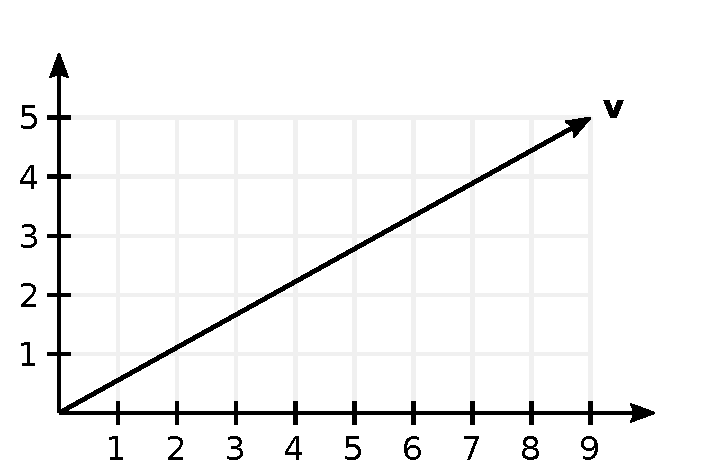
\includegraphics[width=72mm]{img/Vektor.pdf}
\end{center}
\end{frame}

\begin{frame}[t]
\vspace{3em}
Bezüglich einer Basis $A=(\bv a_1,\bv a_2)$ besitzt der
Vektor eine andere Darstellung.\pause

\parspace
Sei z.\,B. $\bv a_1 := \icol{4\\ 1}$ und $\bv a_2 := \icol{1\\ 3}$.%
\pause

\vspace{-1.6em}
\begin{center}
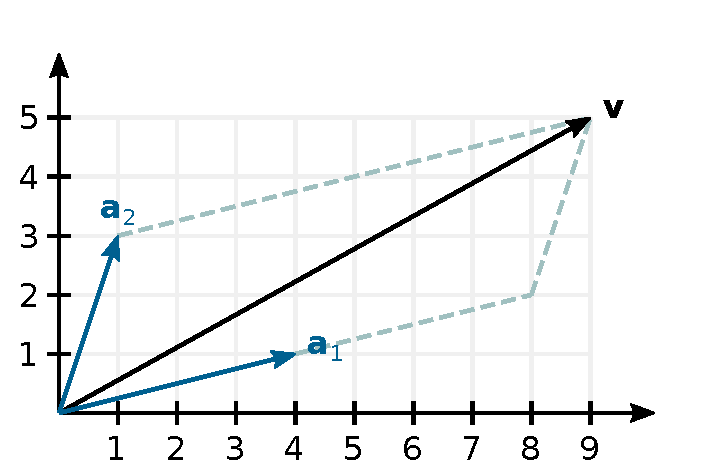
\includegraphics[width=72mm]{img/Vektor-in-Basis-A.pdf}
\end{center}
\end{frame}

\begin{frame}[t]
\vspace{4em}
Bezüglich $A$ besitzt der Vektor die Darstellung
\[\bv v = 2\bv a_1 + 1\bv a_2 = x\bv a_1 + y\bv a_2.
\]\pause
Das Tupel $\bv v_A = (x,y)$ nennen wir \emph{Koordinatenvektor}
zum Vektor $\bv v$ bezüglich Basis $A$.\pause

\parspace
Angenommen, es gibt nun noch eine weitere Basis $B=(\bv b_1,\bv b_2)$.\\
Z.\,B. $\bv b_1:=\icol{7\\ 1}$ und $\bv b_2:=\icol{1\\ 2}$.\pause

\vspace{1.2em}
Wie findet man dann den Koordinatenvektor $\bv v_B=(x',y')$ mit
\[\bv v = x'\bv b_1 + y'\bv b_2?\]
\end{frame}

\begin{frame}
\begin{center}
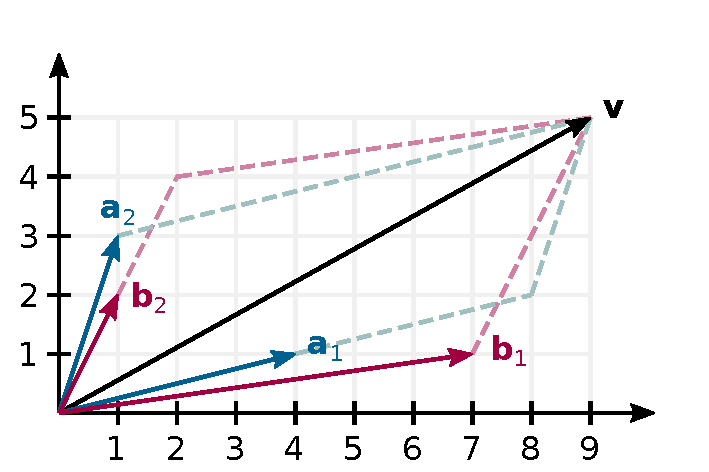
\includegraphics[width=72mm]{img/Vektor-in-Basis-AB.pdf}
\end{center}
\end{frame}

\begin{frame}[t]
\vspace{4em}
Trick: Wir ordnen der Basis
$A=(\begin{pmatrix}a_{11}\\ a_{21}\end{pmatrix},
\begin{pmatrix}a_{12}\\ a_{22}\end{pmatrix})$
die Matrix
\[A=\begin{pmatrix}a_{11} & a_{12}\\ a_{21} & a_{22}\end{pmatrix}\]
zu.\pause{} Dann gilt nämlich
\begin{align*}
\bv v &= x\bv a_1 + y\bv a_2 = x\begin{pmatrix}a_{11}\\ a_{21}\end{pmatrix}
+ y\begin{pmatrix}a_{12}\\ a_{22}\end{pmatrix}\\
&= \begin{pmatrix}a_{11}x + a_{12}y\\ a_{21}x + a_{22}y\end{pmatrix}
= \begin{pmatrix}a_{11} & a_{12}\\ a_{21} & a_{22}\end{pmatrix}\begin{pmatrix}x\\ y\end{pmatrix}
= A\bv v_A.
\end{align*}
\end{frame}

\begin{frame}
Für die Basis $B$ gilt diese Überlegung ebenfalls. Daher ist
\[\bv v = B\bv v_B = A\bv v_A.\]\pause
Weil $B$ eine Basis ist, ist $\det(B)\ne 0$, womit $B$ eine
inverse Matrix $B^{-1}$ besitzt. Multiplizieren wir beide Seiten
der Gleichung von links mit $B^{-1}$, erhalten wir
\[\bv v_B = B^{-1}B\bv v_B = B^{-1}A\bv v_A.\]
Das ist der gesuchte Koordinatenvektor.
\end{frame}

\begin{frame}
\strong{Bemerkung.} Für eine beliebige Matrix
\[B = \begin{pmatrix}b_{11} & b_{12}\\ b_{21} & b_{22}\end{pmatrix}\]
mit $0\ne \det(B) = b_{11}b_{22}-b_{12}b_{21}$ gibt es die Formel
\[B^{-1} = \frac{1}{\det(B)}\begin{pmatrix}
 b_{22} & -b_{12}\\
-b_{21} &  b_{11}
\end{pmatrix}.\]
\end{frame}

\begin{frame}
Anders ausgedrückt ist $B\bv v_B = A\bv v_A$ ein lineares
Gleichungssystem in $\bv v_B=(x',y')$.\pause{} Das ist
\[\begin{pmatrix}b_{11} & b_{12}\\ b_{21} & b_{22}\end{pmatrix}\begin{pmatrix}x'\\ y'\end{pmatrix}
= \begin{pmatrix}a_{11} & a_{12}\\ a_{21} & a_{22}\end{pmatrix}\begin{pmatrix}x\\ y\end{pmatrix}.
\]\pause{}
Im Beispiel ist
\[\begin{pmatrix}7 & 1\\ 1 & 2\end{pmatrix}\begin{pmatrix}x'\\ y'\end{pmatrix}
= \begin{pmatrix}4 & 1\\ 1 & 3\end{pmatrix}\begin{pmatrix}2\\ 1\end{pmatrix}
= \begin{pmatrix}9\\ 5\end{pmatrix}.\]\pause
Das macht $x'=1$ und $y'=2$.
\end{frame}

\begin{frame}
Woher ist eigentlich die Darstellung $\bv v_A$ bekannt?\pause

\parspace
Die bekommen wir auf die gleiche Art.  Die Gleichung
\[\bv v = A\bv v_A\]
müssen wir dazu bloß nach $\bv v_A$ umformen. Man erhält
$\bv v_A = A^{-1}\bv v$.\pause

\parspace
Anders ausgedrückt liegt ein lineares Gleichungssystem
in $\bv v_A$ vor.
\end{frame}

\begin{frame}
\strong{Bemerkung.} Man beachte
\[\bv v = \begin{pmatrix}9\\ 5\end{pmatrix} = 
9\begin{pmatrix}1\\ 0\end{pmatrix} + 5\begin{pmatrix}0\\ 1\end{pmatrix}
= 9\bv e_1 + 5\bv e_2.\]\pause
Die Matrix zur Standardbasis $E=(\bv e_1,\bv e_2)$
ist die Einheitsmatrix
\[E=\begin{pmatrix}1 & 0\\ 0 & 1\end{pmatrix}.
\]\pause
Daher gilt $\bv v = E\bv v_E = \bv v_E$. Das heißt, ein Koordinatenvektor
ist sein eigener Koordinatenvektor. 
\end{frame}

\begin{frame}
\begin{center}
\strong{Kurze Pause}
\end{center}
\end{frame}

\begin{frame}
Nun tauschen wir $\R^2$ gegen einen abstrakten Vektorraum $V$ aus.
Damit ist gemeint, dass nun nicht mehr a priori ein absolutes
Koordinatensystem vorliegt.\pause

\parspace
Dies zieht einige Konsequenzen nach sich. Zum einen existiert für
$\bv v$ keine absolute Darstellung mehr. Zudem sind auch die
Basisvektoren davon betroffen.\pause

\parspace
Da die Matrizen $A$ und $B$ jeweils aus der absoluten Darstellung
ihrer Basisvektoren aufgebaut sind, existieren auch diese nicht mehr.
\end{frame}

\begin{frame}
\begin{center}Vektorraum $\R^2$\end{center}

\vspace{-2em}
\begin{center}
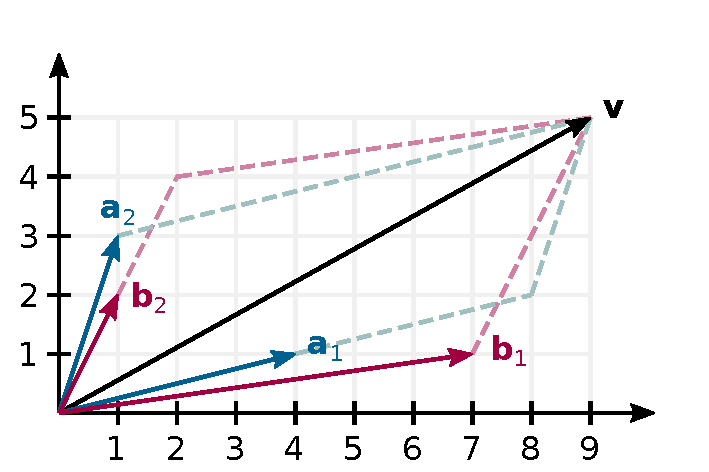
\includegraphics[width=72mm]{img/Vektor-in-Basis-AB.pdf}
\end{center}
\end{frame}

\begin{frame}
\begin{center}Vektorraum $V$\end{center}

\vspace{-2em}
\begin{center}
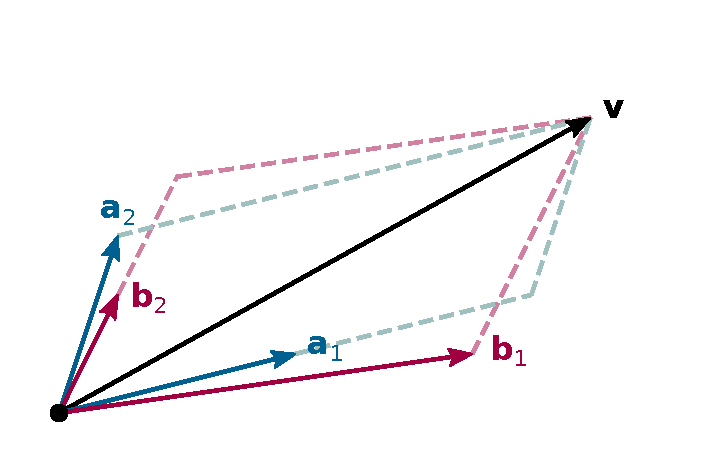
\includegraphics[width=72mm]{img/Abstrakt-in-Basis-AB.pdf}
\end{center}
\end{frame}

\begin{frame}
Was allerdings existiert, ist die Matrix
\[T_B^A := B^{-1}A.\]\pause
Diese Matrix nennen wir \emph{Transformationsmatrix}. Sie wandelt die
Koordinaten von $\bv v$ bezüglich Basis $A$ in die Koordinaten
bezüglich Basis $B$ um.\pause

\parspace
Als Formel:
\[\bv v_B = T_B^A \bv v_A.\]
\end{frame}

\begin{frame}
Wie bekommt man nun aber die Transformationsmatrix, wenn lediglich
eine Beziehung zwischen den Basisvektoren vorliegt? Gegeben sei
die Beziehung
\begin{align*}
\bv a_1 &= s_{11}\bv b_1 + s_{21}\bv b_2,\\
\bv a_2 &= s_{12}\bv b_1 + s_{22}\bv b_2.
\end{align*}\pause
Dies lässt sich in Kurzform schreiben als
\[\bv a_i = \sum_{j=1}^2 s_{ji}\bv b_j.\]
\end{frame}

\begin{frame}
Betrachten wir zur Hilfe kurz noch einmal den $\R^2$.
Da muss gelten
\[a_{ki} = \sum_{j=1}^2 s_{ji}b_{kj}.\]\pause
Aber das ist doch eine Matrizenmultiplikation. Nämlich
\[A^T = S^T B^T\]
mit
\[S = \begin{pmatrix}s_{11} & s_{12}\\
s_{21} & s_{22}\end{pmatrix}.\]
\end{frame}

\begin{frame}
\strong{Jetzt kommt Matrizenrechnung zur Anwendung.}\pause

\vspace{1em}
Transposition auf beiden Seiten der Gleichung bringt
\[A = (S^T B^T)^T = BS.\]\pause
Infolge gilt $S = B^{-1}A$.\pause

\vspace{1em}
Schließlich gelangen wir zu $T_B^A=S$.
\end{frame}

\begin{frame}
Dies verbleibt auch dann gültig, wenn der Vektor $\bv v$
nicht in den Koordinatenraum $\R^2$ eingebettet ist.\pause

\vspace{1em}
\strong{Beweis.} Laut der Beziehung zwischen den Basen gilt
\[\bv v = \sum_{i=1}^2 (\bv v_A)_i\bv a_i
= \sum_{i=1}^2 (\bv v_A)_i\sum_{j=1}^2 s_{ji}\bv b_j
= \sum_{j=1}^2\bigg(\sum_{i=1}^2 s_{ji}(\bv v_A)_i\bigg)\bv b_j,\]
und somit
\[(\bv v_B)_j = \sum_{i=1}^2 s_{ji}(\bv v_A)_i.\pause\]
Kurz $\bv v_B = S\bv v_A$.
Demzufolge gilt $T_B^A = S$.\,\qedsymbol
\end{frame}

\begin{frame}
\strong{Bemerkung.}
Auf die folgende Weise kann man den Beweis in kompakter Form ohne
Indexrechnungen durchführen.\pause

\vspace{1em}
Zwar gibt es die Matrizen $A,B$ nicht mehr, wir können aber dennoch
die linearen Abbildungen $\Phi_A,\Phi_B$ mit
\[\bv v = \Phi_B(\bv v_B) = \Phi_A(\bv v_A)\]
betrachten. Man beachte, dass $\bv a_k = \Phi_A(\bv e_k)$
und $\bv b_k = \Phi_B(\bv e_k)$ gilt. Die Beziehung ist damit
kompakt notierbar als
\[\Phi_A = \Phi_B\circ S.\]\pause
Demzufolge gilt
\[\Phi_B(\bv v_B) = \Phi_A(\bv v_A) = (\Phi_B\circ S)(\bv v_A) = \Phi_B(S\bv v_A).\]
Weil $\Phi_B$ invertierbar ist, darf man $\Phi_B^{-1}$ auf beide
Seiten anwenden. Man erhält wieder $\bv v_B = S\bv v_A$.
\end{frame}

\begin{frame}
Wurde eine ähnliche Rechnung nicht bereits mit Matrizen
durchgeführt?\pause

\vspace{1em}
\strong{Das ist kein Zufall.} Bei Einbettung in den
Koordinatenraum gilt
\begin{align*}
\Phi_A &= A,\\
\Phi_B &= B.
\end{align*}
Das heißt, die Rechnung mit $\Phi_A,\Phi_B$ ist lediglich eine
abstrakte Form der bereits zuvor durchgeführten Rechnung mit
$A,B$.
\end{frame}

\begin{frame}
Umgekehrt ist mit der Einsicht $S = B^{-1}A$ die Beziehung
für das betrachtete Beispiel ermittelbar. Mit
\[S = \begin{pmatrix}7 & 1\\ 1 & 2\end{pmatrix}^{-1}
\begin{pmatrix}4 & 1\\ 1 & 3\end{pmatrix}
= \tfrac{1}{13}\begin{pmatrix}7 & -1\\ 3 & 20\end{pmatrix}\]
findet man
\begin{align*}
\bv a_1 &= \tfrac{7}{13}\bv b_1 + \tfrac{3}{13}\bv b_2,\\
\bv a_2 &= \tfrac{-1}{13}\bv b_1 + \tfrac{20}{13}\bv b_2.
\end{align*}
\end{frame}

\begin{frame}
Ende.
\vfill\hfill\modest{Juni 2021}\\
\hfill\modest{Creative Commons CC0 1.0}
\end{frame}

\end{document}
